%!TEX program = xelatex
\documentclass[11pt,article,oneside]{memoir}

% Disable all warnings issued by biblatex starting with "Since you are using the 'memoir' class..."
\usepackage{silence}
\WarningFilter{biblatex}{Since you are using the}
% And disable the warnings about biblatex and biditools and Arabic
\WarningFilter{biblatex}{File 'arabic-apa.lbx'}
\WarningFilter{biblatex}{Language 'arabic'}
\WarningFilter{biditools}{Patching `\enddocument'}

% Not all fonts have fancy OpenType features like proportional and oldstyle
% figures, so this suppresses fontspec's warnings when using those kinds of fonts
\PassOptionsToPackage{quiet}{fontspec}


% ---------------
% GENERAL SETUP
% ---------------
\usepackage[american]{babel}
\usepackage[babel]{csquotes}
\usepackage{enumitem}
\usepackage{etoolbox}

\setlength{\parindent}{1.5em}


% -------
% FONTS
% -------
% mathtools has \underbracket and \overbracket with options for controlling 
% height and thickness, but unicode-math provides its own option-free versions 
% of these bracket macros. At one point it used to patch these macros and not 
% override mathtools' commands, but it currently does not do that anymore 
% (see https://github.com/wspr/unicode-math/issues/544). 
%
% We use unicode-math here so that we can use custom math fonts with 
% \setmathfont{}, which then messes up bracket options. But there's a solution! 
% We save mathtools' brackets  after loading mathtools, then load 
% unicode-math which clobbers them, and then *after* \begin{document}, redifine 
% the stored brackets (this part is key! According to 
% https://tug.org/pipermail/lualatex-dev/2011-August/001295.html, the unicode 
% table from unicode-math is executed after beginning the document, so 
% redefining the brackets in the preamble won't work)

% Math stuff
\usepackage{amsmath, amssymb, amsfonts, amsthm, mathtools}

% Save mathtools' brackets and braces
\let\normalunderbracket=\underbracket
\let\normaloverbracket=\overbracket

\usepackage{unicode-math}  % For custom math fonts

% Custom fonts
\usepackage{fontspec}
\usepackage{xunicode}
\defaultfontfeatures{Mapping=tex-text,Ligatures=TeX,Scale=MatchLowercase}
\setmainfont[Numbers={Proportional,OldStyle}]{Spectral}
\setsansfont{Open Sans}
\setmonofont[Mapping=tex-ansi, Scale=MatchLowercase]{Inconsolata}
\setmathfont{Libertinus Math}


% ---------------
% TITLE SECTION
% ---------------
% Keywords
\providecommand{\keywords}[1]{\small{\sffamily{\textbf{\textit{Keywords---}}#1 \vskip 3em}}}

% Redefine \and and \andnext to remove tabular environment.
% Needed below for custom article-styles when multiple authors are present.
\renewcommand{\and}{\, }
\renewcommand*{\andnext}{%
  \\\medskip }

% Command for a note at the top of the first page describing the publication
% status of the paper.
\newcommand{\published}[1]{%
   \gdef\puB{#1}}
   \newcommand{\puB}{}
   \renewcommand{\maketitlehooka}{%
       \par\noindent\footnotesize\sffamily \puB}


% --------------------------------
% MEMOIR CHAPTER AND PAGE STYLES
% --------------------------------
% Main style
\makechapterstyle{hikma-article}{
    % Heading 1
    \setsecheadstyle{\Large\sffamily\bfseries}
    \setbeforesecskip{-4.5ex}  % Space before; if negative, next paragraph will not be indented
    \setaftersecskip{1ex}  % Space after

    % Heading 2
    \setsubsecheadstyle{\large\sffamily}
    \setbeforesubsecskip{-2.5ex}
    \setaftersubsecskip{0.7ex}

    % Heading 3
    \setaftersubsubsecskip{-1em}  % Inline heading
    \setsubsubsecheadstyle{\normalsize\sffamily\bfseries}
    \setbeforesubsubsecskip{1.5ex}

    % Captions
    \captiontitlefont{\small\sffamily}
    \captionnamefont{\small\sffamily}
    \subcaptionsize{\small}
    \subcaptionlabelfont{\sffamily}
    \subcaptionfont{\sffamily}

    % TOC stuff
    \settocdepth{subsubsection}
    \maxsecnumdepth{subsubsection}
    \setsecnumdepth{chapter}

    % Change formatting in title block
    \pretitle{\par\vskip 3em \flushleft\LARGE\sffamily\bfseries}
    \posttitle{\par\vskip 0.75em}
    \preauthor{\flushleft\sffamily}
    \postauthor{}
    \predate{\normalsize}
    \postdate{}

    % Abstract stuff
    \renewcommand{\abstractname}{\vspace{-\baselineskip}}  % Remove abstract title
    \renewcommand{\abstracttextfont}{\small\sffamily}

    \epigraphfontsize{\normalfont\footnotesize}
    \setlength\epigraphwidth{186pt}  % 15p6 (31p0 / 2)
    \setlength\epigraphrule{0pt}

    % Footnotes
    \setfootins{3em}{3em}
}

% Numbered article style
\makechapterstyle{hikma-article-numbered} {
  \chapterstyle{hikma-article}  % Copy previous style
  \counterwithout{section}{chapter}  % Make sections start at 1, not 0
  \settocdepth{subsubsection}
  \maxsecnumdepth{subsubsection}
  \setsecnumdepth{subsubsection}
}

% General page style
\makepagestyle{ath}
\makeatletter
\newcommand{\@athmarks}{%
  \let\@mkboth\markboth
  \def\chaptermark##1{%
    \markboth{%
      \ifnum \c@secnumdepth >\m@ne
        \if@mainmatter
          \thechapter. \ %
        \fi
      \fi
      ##1}{}}
  \def\sectionmark##1{%
    \markright{##1}}
}
\makepsmarks{ath}{\@athmarks}
\makepsmarks{ath}{}
% For the first page
\makeevenfoot{plain}{}{\sffamily\footnotesize\thepage}{}
\makeoddfoot{plain}{}{\sffamily\footnotesize\thepage}{}
% For regular pages
\makeevenhead{ath}{}{}{\sffamily\footnotesize\thepage}
\makeoddhead{ath}{}{}{\sffamily\footnotesize\thepage}
\makeatother


% -------------------
% PAGE LAYOUT SUTFF
% -------------------
% For landscape PDF pages
\usepackage{pdflscape}

% For better TOCs
\usepackage{tocloft}

% Treat the TOC title as a section instead of a chapter
\makeatletter
\renewcommand\@tocmaketitle{%
  \section*{\contentsname}
  \tocmark%
  \@afterheading}
\makeatother

% Shift indentation back
% See table showing tocloft's default indents and numwidths
% https://tex.stackexchange.com/a/50472/11851
\cftsetindents{section}{0em}{1.5em}
\cftsetindents{subsection}{1.5em}{2.3em}
\cftsetindents{subsubsection}{3.8em}{3.2em}

% Use sans fonts for all parts of the TOC
\renewcommand{\cftsectionfont}{\normalfont\sffamily}
\renewcommand{\cftsectionpagefont}{\normalfont\sffamily} 
\renewcommand{\cftsubsectionfont}{\normalfont\sffamily}
\renewcommand{\cftsubsectionpagefont}{\normalfont\sffamily}
\renewcommand{\cftsubsubsectionfont}{\normalfont\sffamily}
\renewcommand{\cftsubsubsectionpagefont}{\normalfont\sffamily}

% Page margins
% {left}{right}{ratio} - one has to be *
% 10p0 left/right, 11p0 top/bottom
% Text block is 31p0 wide, 44p0 tall
\setlrmarginsandblock{10pc}{10pc}{*}  % 10p0
\setulmarginsandblock{11pc}{11pc}{*}  % 11p0
\checkandfixthelayout


% ------------------
% TYPOGRAPHY STUFF
% ------------------
% Pandoc tightlists
\providecommand{\tightlist}{%
  \setlength{\itemsep}{0pt}\setlength{\parskip}{0pt}}

% Fix widows and orphans
\usepackage[all,defaultlines=2]{nowidow}

% Add - as an acceptable hyphenation break in URLs
\usepackage{url}
\def\UrlBreaks{\do\.\do\@\do\\\do\/\do\!\do\_\do\|\do\;\do\>\do\]%
    \do\)\do\,\do\?\do\&\do\'\do+\do\=\do\#\do-}

% Ordinarily I'd like to make URLs not monospaced up here with other typographic
% settings, but NOO because if you use apacite, it overwrites whatever
% \urlstyle{} you use, so the actual \urlstyle{same} appears down below in
% the REFERENCES section

% Use "1. Note" in the footnotes
\footmarkstyle{#1.\,}

% Tweak \thanks{} stuff
\thanksheadextra{\small}{}  % Marker in title section
\thanksmarkstyle{\footnotesize #1\,}  % Actual note down in footnotes
\let\oldthanks\thanks
\renewcommand{\thanks}[1]{\oldthanks{\sffamily \footnotesize #1}}

% Wrap definition list terms
% https://tex.stackexchange.com/a/9763/11851
\setlist[description]{style=unboxed}

% Fancier verbatims
\usepackage{fancyvrb}

% Hyperlink stuff
\usepackage[xetex, colorlinks=true, urlcolor=DarkSlateBlue,
            citecolor=DarkSlateBlue, filecolor=DarkSlateBlue, plainpages=false,
            pdfpagelabels, bookmarksnumbered]{hyperref}

% Color names for hyperlinks
\usepackage[svgnames]{xcolor}

% Syntax highlighting stuff


% --------
% MACROS
% --------
\newcommand{\blandscape}{\begin{landscape}}
\newcommand{\elandscape}{\end{landscape}}
\newcommand{\stgroup}{\begingroup}
\newcommand{\fingroup}{\endgroup}

\DisemulatePackage{setspace}
\usepackage{setspace}

\newcommand{\memSingle}{\setSingleSpace{1.15}\SingleSpacing}
\newcommand{\memSingleSmall}{\setSingleSpace{0.9}\SingleSpacing}

% --------
% TABLES
% --------
\usepackage{booktabs}
\usepackage{longtable}
\usepackage{pbox}  % For multi-line table cells

% Things that kableExtra needs
\usepackage{array}
\usepackage{multirow}
\usepackage{wrapfig}
\usepackage{float}
\usepackage{colortbl}
\usepackage{tabu}
\usepackage{threeparttable}
\usepackage{threeparttablex}
\usepackage[normalem]{ulem}
\usepackage{makecell}
\usepackage{xcolor}

% Make tables sans serif
\setfloatadjustment{table}{\footnotesize\sffamily}
% memoir's setfloatadjustment doesn't work on longtables, but this does
\AtBeginEnvironment{longtable}{\footnotesize\sffamily}

% Remove left margin in lists inside longtables
% https://tex.stackexchange.com/a/378190/11851
\AtBeginEnvironment{longtable}{\setlist[itemize]{nosep, wide=0pt, leftmargin=*, before=\vspace*{-\baselineskip}, after=\vspace*{-\baselineskip}}}


% ----------
% GRAPHICS
% ----------
\usepackage{graphicx}
\makeatletter
\def\maxwidth{\ifdim\Gin@nat@width>\linewidth\linewidth\else\Gin@nat@width\fi}
\def\maxheight{\ifdim\Gin@nat@height>\textheight\textheight\else\Gin@nat@height\fi}
\makeatother
% Scale images if necessary, so that they will not overflow the page
% margins by default, and it is still possible to overwrite the defaults
% using explicit options in \includegraphics[width, height, ...]{}
\setkeys{Gin}{width=\maxwidth,height=\maxheight,keepaspectratio}


% --------------
% I18N SUPPORT
% --------------
% This has to come before loading biblatex
\usepackage{polyglossia}
\setdefaultlanguage{english}
% \setotherlanguage{arabic}
% \newfontfamily\arabicfont[Script = Arabic]{Amiri}


% ------------
% REFERENCES
% ------------
% NB: Using "strict" messes with footnotes and removes the rule!

\usepackage[authordate, backend=biber, noibid,
            autolang=hyphen, bibencoding=inputenc,
            isbn=false, uniquename=false]{biblatex-chicago} % biblatex setup

% No space between bib entries + use smaller font
\setlength\bibitemsep{0pt}
\renewcommand*{\bibfont}{\footnotesize}

%% Fix biblatex's odd preference for using In: by default.
\renewbibmacro{in:}{%
  \ifentrytype{article}{}{%
  \printtext{\bibstring{}\intitlepunct}}}

%% bibnamedash: with Minion Pro the three-emdash lines in the
%% bibliogrpaphy end up separated from one another, which is very
%% annoying. Replace them with a line of appropriate size and weight.
\renewcommand{\bibnamedash}{\rule[3.5pt]{3em}{0.5pt}}

\addbibresource{references.bib}
\setlength\bibhang{\parindent}

% Don't typeset URLs in a monospaced font
% This has to come after apacite because apacite sets its own URL style
\urlstyle{same}


% ----------
% METADATA
% ----------
% Add PDF metadata
\hypersetup{pdfinfo={
  Title={Example paper from R Markdown},
  Author={Author 1, Author 2},
  Creator={R Markdown, pandoc, and TeX},
  Keywords={k1; k2; k3}
  % Subject={},
}}

% Add content from pandoc metadata
\title{\bigskip \bigskip Example paper from R Markdown\thanks{I thank
\(x\), \(y\). Financial support from \(z\) is greatly acknowledged.}}

\author{
  \large Author 1 \newline
  \footnotesize University of Whatever \newline
  \footnotesize \url{author1@example.ac.uk}\vspace*{1.1em}\newline
    \and
  \large Author 2 \newline
  \footnotesize University of Wherever \newline
  \footnotesize \url{author2@example2.ac.uk}\vspace*{1.1em}\newline
  }

\date{}


% ---------------------
% RESPONSE MEMO STUFF
% ---------------------


% -------------------
% STUFF FROM PANDOC
% -------------------
\makeatletter
\@ifpackageloaded{subfig}{}{\usepackage{subfig}}
\@ifpackageloaded{caption}{}{\usepackage{caption}}
\captionsetup[subfloat]{margin=0.5em}
\AtBeginDocument{%
\renewcommand*\figurename{Figure}
\renewcommand*\tablename{Table}
}
\AtBeginDocument{%
\renewcommand*\listfigurename{List of Figures}
\renewcommand*\listtablename{List of Tables}
}
\newcounter{pandoccrossref@subfigures@footnote@counter}
\newenvironment{pandoccrossrefsubfigures}{%
\setcounter{pandoccrossref@subfigures@footnote@counter}{0}
\begin{figure}\centering%
\gdef\global@pandoccrossref@subfigures@footnotes{}%
\DeclareRobustCommand{\footnote}[1]{\footnotemark%
\stepcounter{pandoccrossref@subfigures@footnote@counter}%
\ifx\global@pandoccrossref@subfigures@footnotes\empty%
\gdef\global@pandoccrossref@subfigures@footnotes{{##1}}%
\else%
\g@addto@macro\global@pandoccrossref@subfigures@footnotes{, {##1}}%
\fi}}%
{\end{figure}%
\addtocounter{footnote}{-\value{pandoccrossref@subfigures@footnote@counter}}
\@for\f:=\global@pandoccrossref@subfigures@footnotes\do{\stepcounter{footnote}\footnotetext{\f}}%
\gdef\global@pandoccrossref@subfigures@footnotes{}}
\@ifpackageloaded{float}{}{\usepackage{float}}
\floatstyle{ruled}
\@ifundefined{c@chapter}{\newfloat{codelisting}{h}{lop}}{\newfloat{codelisting}{h}{lop}[chapter]}
\floatname{codelisting}{Listing}
\newcommand*\listoflistings{\listof{codelisting}{List of Listings}}
\makeatother


% ------------------------------------------------------------------------------
% ------------------------------------------------------------------------------
% ------------------------------------------------------------------------------

% ----------------
% ACTUAL DOCUMENT
% ----------------

\begin{document}

% Restore mathtools' brackets *after* \begin{document}
\let\underbracket=\normalunderbracket
\let\overbracket=\normaloverbracket

\chapterstyle{hikma-article}
\pagestyle{athgit}

% Otherwise, use the normal article title + abstract + epigraph
\published{\textbf{07 February, 2022} \qquad Working
paper. \\ {\tiny Access the code at
\url{https://github.com/ygalanak/DataAnalysisTemplate}}}

\maketitle


\begin{abstract}
\noindent Lorem ipsum dolor sit amet, consectetur adipisicing elit, sed
do eiusmod tempor incididunt ut labore et dolore magna aliqua. Ut enim
ad minim veniam, quis nostrud exercitation ullamco laboris nisi ut
aliquip ex ea commodo consequat. Duis aute irure dolor in reprehenderit
in voluptate velit esse cillum dolore eu fugiat nulla pariatur.
Excepteur sint occaecat cupidatat non proident, sunt in culpa qui
officia deserunt mollit anim id est laborum
\bigskip
\end{abstract}

\keywords{k1; k2; k3}




\hypertarget{introduction}{%
\section{Introduction}\label{introduction}}

Lorem ipsum dolor sit amet, consectetur adipisicing elit, sed do eiusmod
tempor incididunt ut labore et dolore magna aliqua
\autocite{HeissKelley:2017}. Ut enim ad minim veniam, quis nostrud
exercitation ullamco laboris nisi ut aliquip ex ea commodo consequat
\autocite{KeckSikkink:1998}. Duis aute irure dolor in reprehenderit in
voluptate velit esse cillum dolore eu fugiat nulla pariatur
\autocite{Heiss:2019}.

\begin{figure}
\hypertarget{fig:mpg-plot}{%
\centering
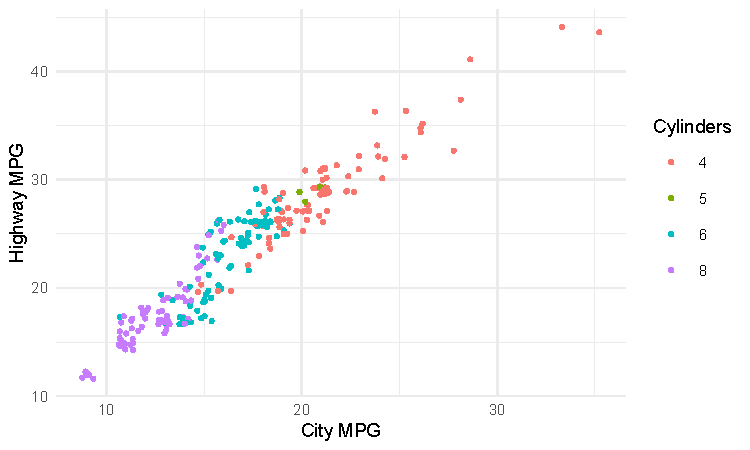
\includegraphics{./figs-tbls/mpg-plot.pdf}
\caption{Scatterplot showing the relationship between city and highway
miles per gallon}\label{fig:mpg-plot}
}
\end{figure}

Sed ut perspiciatis unde omnis iste natus error sit voluptatem
accusantium doloremque laudantium, totam rem aperiam (see
Figure~\ref{fig:mpg-plot}), eaque ipsa quae ab illo inventore veritatis
et quasi architecto beatae vitae dicta sunt explicabo.

\[ 
\text{This is a test} = \beta_1 x_1 + \epsilon 
\]

Nemo enim ipsam voluptatem quia voluptas sit aspernatur aut odit aut
fugit, sed quia consequuntur magni dolores eos qui ratione voluptatem
sequi nesciunt.

\hypertarget{new-section}{%
\section{New section}\label{new-section}}

Neque porro quisquam est, qui dolorem ipsum quia dolor sit amet,
consectetur, adipisci velit, sed quia non numquam eius modi tempora
incidunt ut labore et dolore magnam aliquam quaerat voluptatem. Ut enim
ad minima veniam, quis nostrum exercitationem ullam corporis suscipit
laboriosam, nisi ut aliquid ex ea commodi consequatur?

\hypertarget{subsection}{%
\subsection{Subsection}\label{subsection}}

In Table~\ref{tbl:mytable}, quis autem vel eum iure reprehenderit qui in
ea voluptate velit esse quam nihil molestiae consequatur, vel illum qui
dolorem eum fugiat quo voluptas nulla pariatur?

\hypertarget{tbl:mytable}{}
\begin{longtable}[]{@{}
  >{\centering\arraybackslash}p{(\columnwidth - 2\tabcolsep) * \real{0.1389}}
  >{\centering\arraybackslash}p{(\columnwidth - 2\tabcolsep) * \real{0.2222}}@{}}
\caption{\label{tbl:mytable}This is a table}\tabularnewline
\toprule
\begin{minipage}[b]{\linewidth}\centering
Heading
\end{minipage} & \begin{minipage}[b]{\linewidth}\centering
Other heading
\end{minipage} \\
\midrule
\endfirsthead
\toprule
\begin{minipage}[b]{\linewidth}\centering
Heading
\end{minipage} & \begin{minipage}[b]{\linewidth}\centering
Other heading
\end{minipage} \\
\midrule
\endhead
2 & 3 \\
5 & 7 \\
9 & 1 \\
\bottomrule
\end{longtable}

At vero eos et\footnote{This is a footnote with an in-text reference
  \textcite{HeissKelley:2017}.} accusamus et iusto odio dignissimos
ducimus qui blanditiis praesentium voluptatum deleniti atque corrupti
quos dolores et quas molestias excepturi sint occaecati cupiditate non
provident, similique sunt in culpa qui officia deserunt mollitia animi,
id est laborum et dolorum fuga. Et harum quidem rerum facilis est et
expedita distinctio.

\hypertarget{subsection-again}{%
\subsection{Subsection again}\label{subsection-again}}

Nam libero tempore, cum soluta nobis est eligendi optio cumque nihil
impedit quo minus id quod maxime placeat facere possimus, omnis voluptas
assumenda est\footnote{This is a footnote.}, omnis dolor repellendus.
Temporibus autem quibusdam et aut officiis debitis aut rerum
necessitatibus saepe eveniet ut et voluptates repudiandae sint et
molestiae non recusandae. Itaque earum rerum hic tenetur a sapiente
delectus, ut aut reiciendis voluptatibus maiores alias consequatur aut
perferendis doloribus asperiores repellat.

\hypertarget{conclusion}{%
\section{Conclusion}\label{conclusion}}

\hypertarget{this-comes-from-another-file}{%
\subsection{This comes from another
file}\label{this-comes-from-another-file}}

Lorem ipsum dolor sit amet, consectetur adipisicing elit, sed do eiusmod
tempor incididunt ut labore et dolore magna aliqua. Ut enim ad minim
veniam, quis nostrud exercitation ullamco laboris nisi ut aliquip ex ea
commodo consequat. Duis aute irure dolor in reprehenderit in voluptate
velit esse cillum dolore eu fugiat nulla pariatur. Excepteur sint
occaecat cupidatat non proident, sunt in culpa qui officia deserunt
mollit anim id est laborum.

Sed ut perspiciatis unde omnis iste natus error sit voluptatem
accusantium doloremque laudantium, totam rem aperiam, eaque ipsa quae ab
illo inventore veritatis et quasi architecto beatae vitae dicta sunt
explicabo. Nemo enim ipsam voluptatem quia voluptas sit aspernatur aut
odit aut fugit, sed quia consequuntur magni dolores eos qui ratione
voluptatem sequi nesciunt. Neque porro quisquam est, qui dolorem ipsum
quia dolor sit amet, consectetur, adipisci velit, sed quia non numquam
eius modi tempora incidunt ut labore et dolore magnam aliquam quaerat
voluptatem. Ut enim ad minima veniam, quis nostrum exercitationem ullam
corporis suscipit laboriosam, nisi ut aliquid ex ea commodi consequatur?
Quis autem vel eum iure reprehenderit qui in ea voluptate velit esse
quam nihil molestiae consequatur, vel illum qui dolorem eum fugiat quo
voluptas nulla pariatur?

\printbibliography[heading=subbibliography, title=References]


\end{document}
